\newenvironment{rcases} {\left.\begin{aligned}} {\end{aligned}\right\rbrace}

\chapter{An Introduction to DFTB Parameterization}
\label{chap:intro}

\section{DFTB}

\textbf{Expansion from DFT\\}
\begin{equation} 
\begin{aligned}
  E&[\rho^0(r)+\Delta\rho(r)] =
    {\color{black}
    \begin{rcases}
      \sum_i^{occ}\langle\psi_i|H^0|\psi_i\rangle 
    \end{rcases}E^{BS}}\\
    &{\color{blue}
    \begin{rcases}
      &-\frac{1}{2}\int\int\frac{\rho^0(r')\rho^0(r)}{|r-r'|}dr'dr -\int v^{xc}[\rho^0(r)]\rho^0(r)dr\\
      &+ E^{xc}[\rho^0(r)] + E^{NN}
    \end{rcases}\approx\frac{1}{2}\sum_{a,b}V^{rep}_{ab}(R_{ab})=E^{rep}}\\
    &{\color{cyan}
    \begin{rcases}
     +\frac{1}{2}\int\int \bigg ( \frac{1}{|r-r'|} + \frac{\delta^2 E^{xc}[\rho(r)]}
     {\delta\rho(r')\delta\rho(r)} \big|_{\rho^0(r')\rho^0(r)} \bigg ) \Delta \rho(r')\Delta \rho(r) dr'dr \\
    \end{rcases}E^{2nd}}\\
    &{\color{orange}
    \begin{rcases}
       &+\frac{1}{6}\int\int\int \bigg ( \frac{\delta^3 E^{xc}[\rho(r)]}{\delta\rho(r'')\delta\rho(r')\delta\rho(r)} \big|_{\rho^0(r'')\rho^0(r')\rho^0(r)} \bigg ) \\
       &\Delta \rho(r'') \Delta \rho(r')\Delta \rho(r)  dr''dr'dr
    \end{rcases}E^{3rd}}\\
    &  +\dots.
\end{aligned}
\label{eq:edftexpand}
\end{equation}

\textbf{None Consistent-Charge (NCC)-DFTB\\}
\begin{equation} 
  E^{NCC-DFTB}=\sum_i^{occ}\langle\psi_i|H^0|\psi_i\rangle + E^{rep}.
  \label{eq:nccdftb}
\end{equation}
Eigenvalue problem:
\begin{equation} 
  \sum_\nu^{AO}c_{\nu i}(H^0_{\mu\nu}-\epsilon_iS_{\mu\nu})= 0.
\end{equation}
Hamiltonian matrix elements, $H^0_{\mu\nu}$:
\begin{equation} 
  H^0_{\mu\nu}=
  \begin{cases}
    \big\langle\phi_\mu\big|-\frac{1}{2}\nabla^2+V[\rho^0_a+\rho^0_b]\big|\phi_\nu\big\rangle& \text{if } a \ne b \\
    \epsilon^{\text{free atom}}                                                            & \text{if } a=b, \mu = \nu\\
    0                                                                                      & \text{if } a=b, \mu \ne \nu.
  \end{cases}
\end{equation}

\textbf{Self-Consistent-Charge (SCC)-DFTB\\}
\begin{equation} 
  E^{SCC-DFTB}=\sum_i^{occ}\langle\psi_i|H^0|\psi_i\rangle {\color{blue}+ E^{rep}} {\color{cyan} + \frac{1}{2}\sum_{a,b}\gamma_{ab}(R_{ab})\Delta q_a \Delta q_b}.
  \label{eq:sccdftb}
\end{equation}
Eigenvalue problem:  
\begin{equation} 
  \sum_\nu^{AO}c_{\nu i}(H_{\mu\nu}-\epsilon_iS{\mu\nu})= 0,
  \label{eq:eigsccdftb}
\end{equation}
Hamiltonian, $H_{\mu\nu}$:
\begin{equation} 
  H_{\mu\nu} = H^0_{\mu\nu} + \frac{1}{2}S_{\mu\nu}\sum_{c}(\gamma_{ac}+\gamma_{bc})\Delta q_c.
\end{equation}
 Mulliken charge, $\Delta$q :
  \begin{equation}
    \Delta q_a = \frac{1}{2}\sum_i n_i \sum_{\mu\in a}\sum_{\nu}(c_{\mu i}c_{\nu i}S_{\mu\nu}+c_{\nu i}c_{\mu i}S_{\nu\mu})
      -q_a^0,
  \end{equation}
$\Delta q_c$ depends on MO coefficients $\Rightarrow$ must be solved iteratively.

\section{Electronic Parameters}

\begin{itemize}
  \item Minimal basis set:
    \subitem Pure atomic orbitals (AOs) are too diffuse%\n $\Rightarrow$ need to be reopitimized.
  \item Electron density $\rho^o$:
    \subitem  $\rho$ is more compressed in molecule
\end{itemize} 

\begin{figure}[H]
  \centering
  \label{fig:h2}
  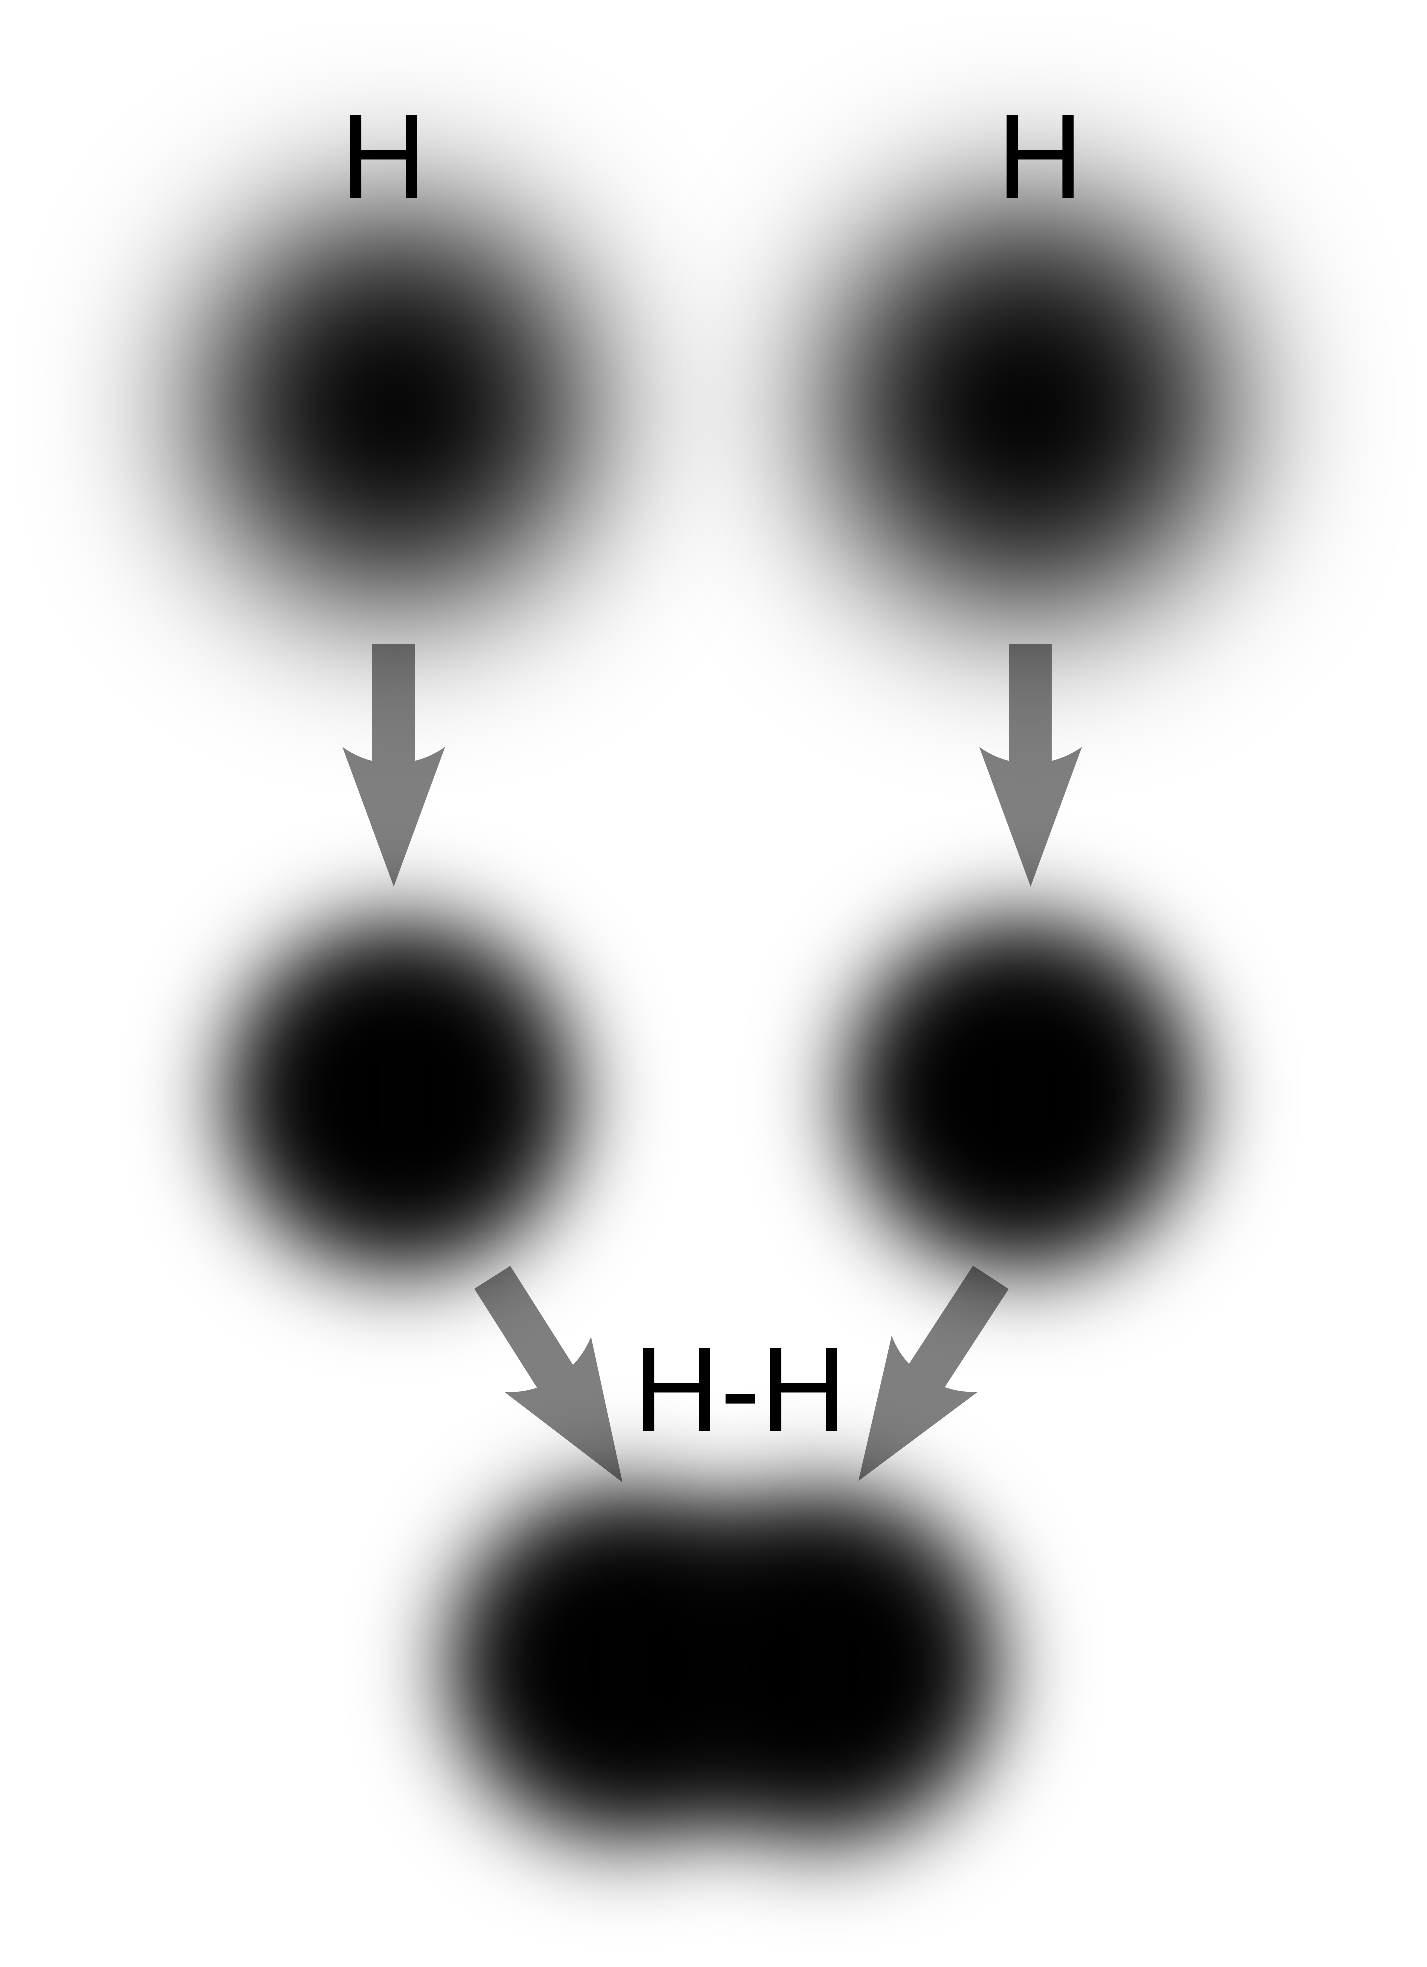
\includegraphics[scale=0.2,angle=0]{h2.eps}
  %\label{fig:h2}
\end{figure}

\begin{equation} 
  \Rightarrow  \Bigg[ -\frac{1}{2}\nabla^2 + v^{eff} [ \rho^{atom} ] {\color{red} + \Bigg(\frac{r}{r_o}\Bigg)^2} \Bigg]\phi_\mu=\epsilon_\mu\phi_\mu 
\end{equation}
\begin{itemize}
  \item[] Free variables:
    \subitem Minimal AO basis set $\Rightarrow r_o^{wf}$
    \subitem Electron density $\rho^o$ $\Rightarrow r_o^{dens}$
\end{itemize}

\section{Repulsive Potentials}

Repulsive Potentials $E^{rep}$: sum of two-center repulsions,
\begin{equation}
E^{rep} = \frac{1}{2} \sum_{A,B} V_{AB}(|\mathbf{R}_A-\mathbf{R}_B|),
\label{ErepAB}
\end{equation} 
Where,
\begin{equation} 
\begin{aligned}
  V_{AB}(R_{AB})=
  \begin{cases}
    e^{-a_1*R_{AB}+a_2} + a_3,  \quad &R_{AB}<R_{AB,0},\\
    \sum_{i=0}^4 a_{AB,n,i} (R_{AB}-R_{AB,n})^i,  \quad &R_{AB,n}\leq R_{AB}<R_{AB,n+1}; 4 \le n \le 6\\
    0,  \quad &R_{AB,cut-off}\leq R_{AB},
  \end{cases}
\end{aligned}
\label{spline}
\end{equation}

Free variables: $R_{AB,n}$ and $a_{AB,n,i}$.

\section{Scoring Function}

\begin{equation} 
\begin{aligned}
  f^{score}=&\sum_{i\in equi} W_{at,i}\left|E^{ref}_{at,i}-E^{DFTB}_{at,i}\right| + \sum_{i\in bar} W_{bar,i}\left|E^{ref}_{bar,i}-E^{DFTB}_{bar,i}\right|\\
%          +&\sum_{i\in equi} \frac{W_{f,i}}{3N_i}\sum_{j\in 3N_i} \left|F^{DFTB}_{i,j}\right| + \sum_{i\in pert} \frac{W_{f,i}}{3N_i}\sum_{j\in 3N_i} \left|F^{ref}_{i,j}-F^{DFTB}_{i,j}\right|,
           +&\sum_{i\in equi} W_{f,i}\sum_{j\in 3N_i} \left|F^{DFTB}_{i,j}\right| + \sum_{i\in pert} W_{f,i}\sum_{j\in 3N_i} \left|F^{ref}_{i,j}-F^{DFTB}_{i,j}\right|,
\label{fscore}
\end{aligned}
\end{equation}\\
\vspace{0.5in}
$W_{at,i}, W_{bar,i}, W_{f,i}$:  Weight factors\\   
$E_{at}$: Atomization energies\\ 
$E_{bar}$: Proton transfer barriers\\  
$N$: Number of atoms\\
$F$: Forces\\  

\pagebreak
\section{Genetic Algorithm}
\begin{figure}[H]
  \centering
  \label{fig:ga}
  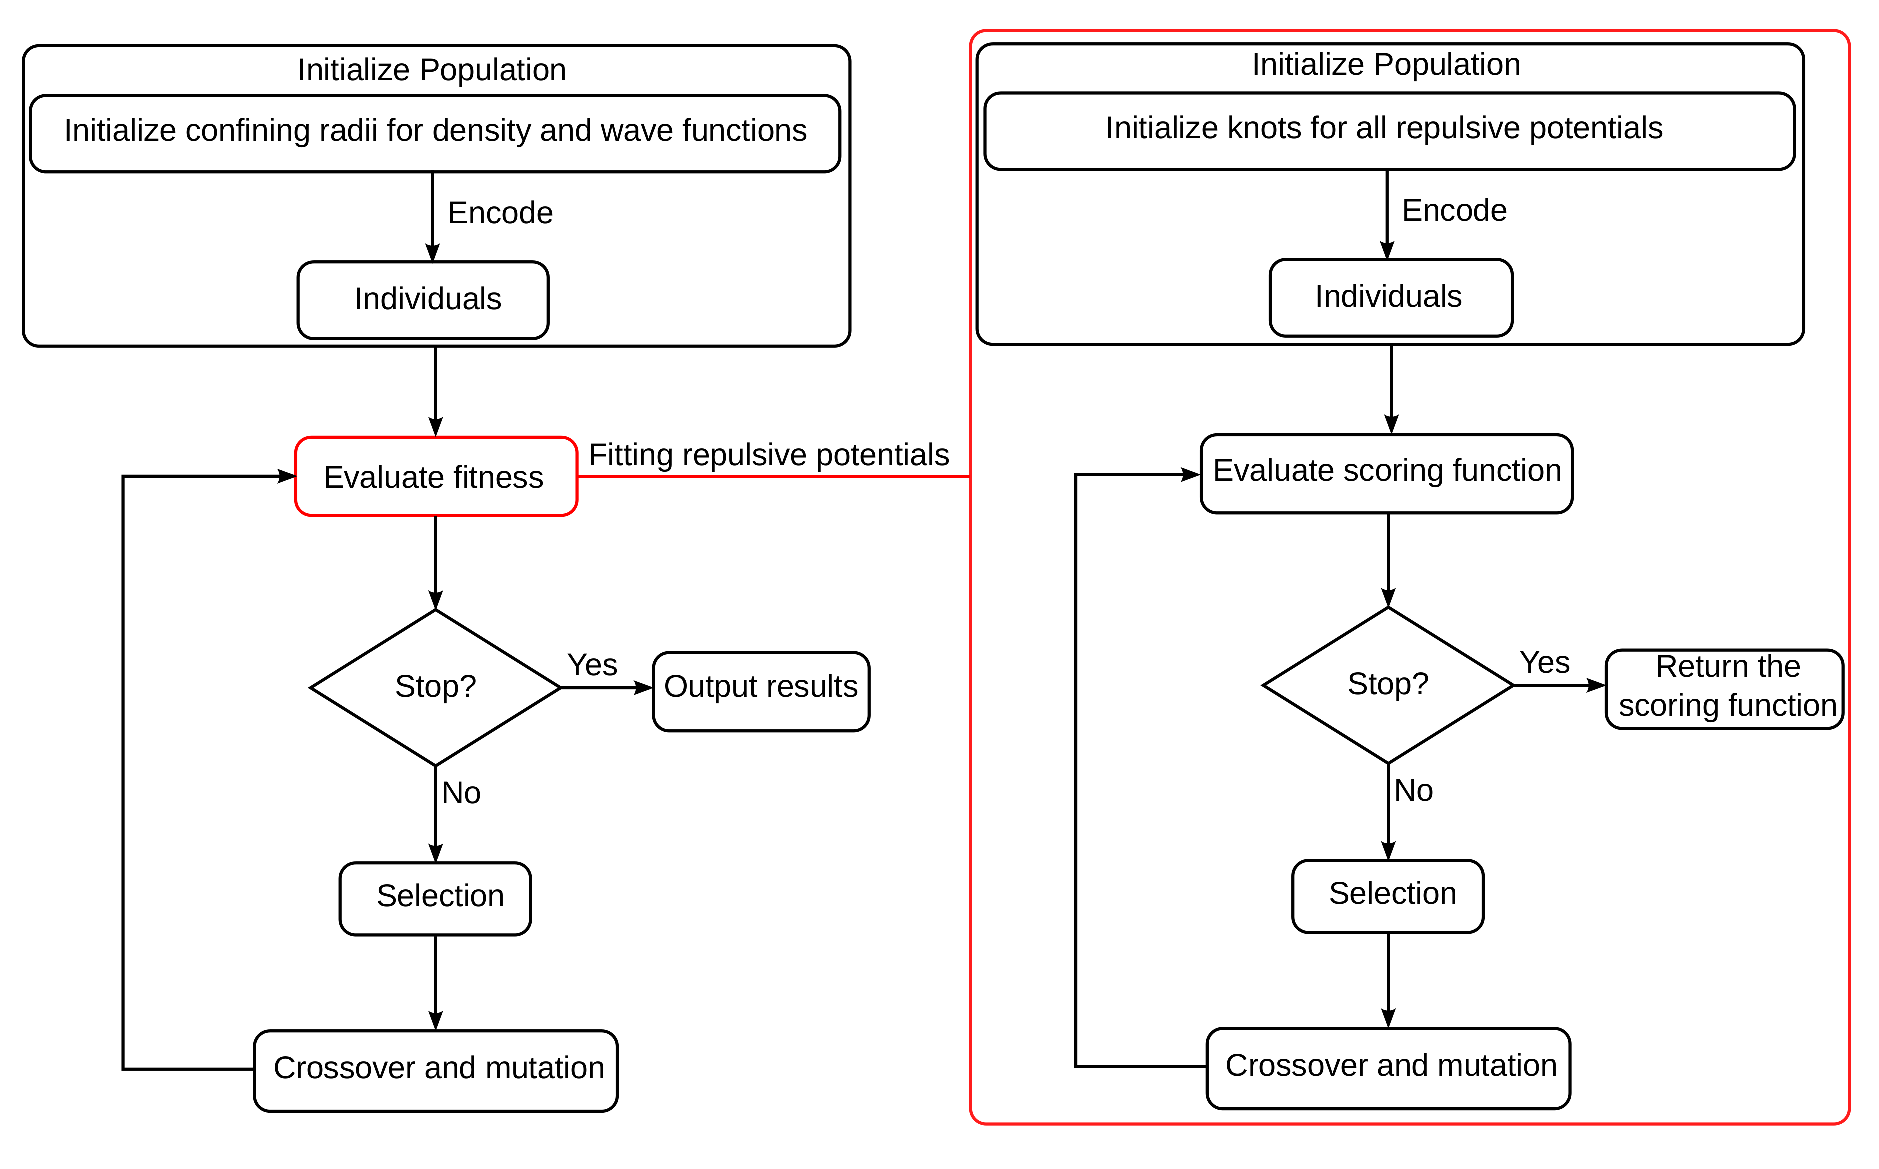
\includegraphics[scale=0.5, angle=0]{ga.eps}
\end{figure}

